% !TeX root = root.tex
% !TeX spellcheck = en_US
\section{GAP-exercise}
Let $G = \langle (3,5,7)(1,2,4), (1,8,3,4,2), (1,2,3,4,5) \rangle$ be a subgroup of $S_8$. Then with the following GAP code we obtain that the order of $G$ is $2520 = \frac{7!}{2}$. Moreover, $G$ is the alternating group over $1,2,3,4,5,7,8$ and is therefore isomorphic to $A_7$.


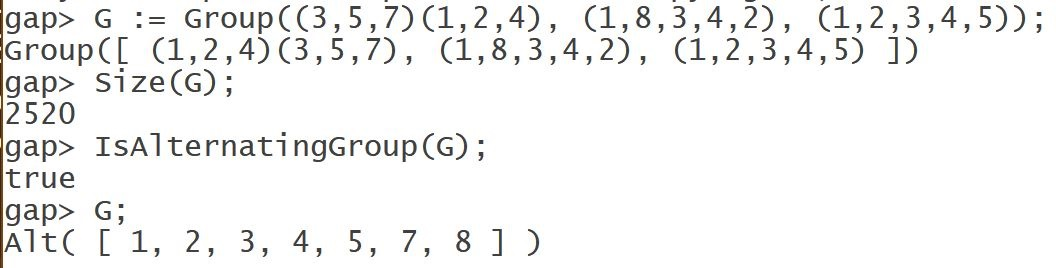
\includegraphics[width=10cm]{gap_code}